\documentclass[runningheads,a4paper]{llncs}
\usepackage{color}
\usepackage{amssymb}
\usepackage{amsmath}
\usepackage{tikz}
\usepackage{pgfplots}
\usetikzlibrary{positioning}
\usetikzlibrary{calc}
\usetikzlibrary{arrows.meta, automata, positioning, calc}
\usepackage{xcolor}
\usepackage{pgf}
\usepackage{tikz}
\usetikzlibrary{arrows,automata,calc}

\newcommand{\locend}{\ensuremath{l_\mathit{End}}}

\begin{document}

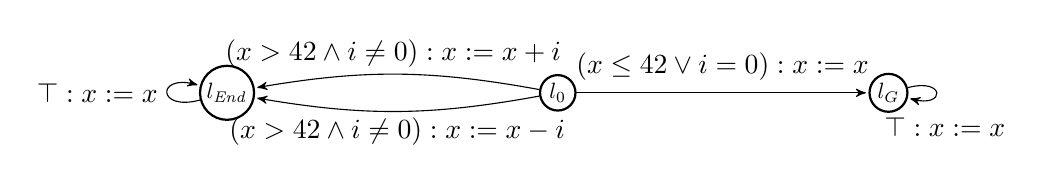
\begin{tikzpicture}[->,>=stealth',shorten >=1pt,auto,node distance=2.5cm]
  \tikzstyle{every state}=[fill=none,draw=black,text=black,inner sep=1.5pt, minimum size=16pt,thick,scale=0.8]
    \node[state] (l) at (0,0) {$l_0$};
    \node[state] (lE) at (-4.2,0) {$\locend$};
    \node[state] (lG) at (4.2, 0) {$l_G$};
    \path (l) edge[bend left=10] node[above, yshift=.4cm] 
              {$\begin{array}{c}(x > 42 \land i \neq 0): x := x + i\;\end{array}$} (lE)
          (l) edge[bend right=10] node[below, yshift=-.4cm] 
              {$\begin{array}{c}(x > 42 \land i \neq 0) : x := x - i\end{array}$} (lE)
          (l) edge node[above] {$\begin{array}{c}(x \leq 42 \lor i = 0): x := x\end{array}$} (lG)
          (lG) edge[loop right] node[below, near end,yshift=-.1cm,xshift=.2cm] {$\top: x := x$} (lG)
           (lE) edge[loop left] node[left] {$\top: x := x$} (lE);
\end{tikzpicture}

\end{document}